\section{Experiments}
\label{sec:eval}

%The following experiments are needed for ACL submission:
%\begin{itemize}
%  \item KBC evaluation on standard dataset. This is what we've done
%        now. We need to show that our schema-base approach performs
%		as good as state-of-the-art.
%  \item KBC evaluation on biased dataset. We need to eyeball PATTY
%        relations and select those complex relations. Then we can
%		compare skeleton-based and schema-based approach.
%  \item QA evalution on biased dataset. Based on complex relations,
%        we find factoid questions (and make some simple modifications
%		if needed) from Yahoo! Answers. And we need to find a way
%		to plug our model in some existing QA systems.
%  \item Relation simialrity dataset to show the expressiveness of
%        compact and human-readable representations, instead of
%		massive features or purely data-driven model. 
%		We first extract PPDB relation pairs and eyeball selecting 
%		good pairs (no same stemmings in PPDB and corresponding 
%		relations in PATTY could get enough entity pairs).
%		This time, ``co-occurrence $\geq$ 1'' should be removed, 
%		otherwise we couldn't find enough pairs.
%		Baselines could be word-based w2v, or simply counting EP
%		overlap between different PATTY relation instances.
%\end{itemize}
%
%And we have a list of ablation tests:
%\begin{itemize}
%  \item What's the result if we won't add any constraints?
%  \item What's the result if we change a naive labeling function?
%        Maybe version 4, version 1 and naive ``positive ratio + 
%		negative ratio'' could be baselines.
%  \item What's are the running times and results when we change a
%        different budget?
%  \item (Optional) compare the results generated from different
%        negative entity pairs. Maybe some generating strategy can
%		show a better difference of results between skeleton-based
%		and schema-based methods.
%\end{itemize}
%

In this section, we evaluate the schemas learned from input NL relations. 
We first evaluate the performance on the knowledge
base completion (KBC) task where the relations come from an Open IE system,
then we compare with state-of-the-art systems on question answering
task using questions involving complex relations. 
Finally, we show that our schema representation can be used to compute
similarity between NL relations and achieve comparable results against
word embedding models.


\subsection{Experiment Setup}
In our experiments, we use the data extracted
by PATTY \cite{nakashole2012patty}, an Open IE system. 
PATTY contains more than 200,000 different relations with
millions of entity pairs extracted from Wikipedia.
%To evaluate the quality of paraphrasing, we build two relation datasets containing 
%positive and negative $\langle e_1, r, e_2 \rangle$ relation triples, and perform
%paraphrasing task over Freebase.
Our KB is a subset of the Freebase dump (June 2015) as our knowledge base.
We pick the top 3,000,000 unique entities by popularity (by counting total
number of triples that an entity appears in), 
along with intermediate entities that connect at least 2 popular entities. 
All direct edges between these entities
and all isa relations connected to these entities are retained in our KB.
\tabref{tab:fb-size} shows the size of this knowledge base.
For experiments in this section, we set the following parameters: 
$\tau$ = 3, $\gamma$ = 10\%, and size of the
priority queue is 1000.


\begin{table}[ht]
\small
	\centering
	\caption{Statistics our KB (subset of Freebase)}
	\begin{tabular}{|c|c|}
		%\toprule
        \hline
		Ordinary Entities	 & 3,000,000 \\
        \hline
        Mediator entities & 7,301,261 \\
		\hline
		Total Entities & 10,301,261 \\
		\hline
		Distinct Relations & 4,412 \\
        \hline
		Types & 2,063 \\
		\hline
	\end{tabular}%
	\label{tab:fb-size}%
\end{table}

\subsection{KBC Evaluation on Complex Relations}
We first evaluate knowledge base completion (KBC) on complex relations 
to see how much gain a schema-based approach can attain. 
KBC task takes training relation instances as input, and predict
whether a new entity pair belongs to one particular relation or not.
We annotated gold schemas for 1,077 distinct PATTY relations which
have at least 100 relation instances,
and in total 61 complex relations are selected for this evaluation. 
\tabref{tab:complex-example} shows some example relations with
labeled schemas.

\begin{table}[ht]
\small
	\centering
	\caption{Example complex relations and their schemas.}
	\begin{tabular}{|c|c|}
		\hline
		Relation		& Schema	\\
        \hline
        \hline
		be county of	& contained\_by + IsA($x_{subj}$)=us\_county \\
        \hline
		be nephew of 	& \pbox{20cm}{parents + siblings + \\ gender($x_{subj}$)=male} \\
		\hline
        professor at	& \pbox{20cm}{employment\_history + at\_company \\  + IsA($x_{obj}$)=university} \\
		\hline
		\pbox{10cm}{died from \\ heart attack in}	& \pbox{20cm}{place\_of\_death + \\ cause\_of\_death($x_{subj}$)=heart\_disease} \\
		\hline
		\pbox{10cm}{play colledge \\ baseketball in} & \pbox{20cm}{athelete\_played + in\_sports\_team + 
				\\ belong\_to\_school + sport($x_2$)=basketball}	\\
		\hline
		study art in	& \pbox{20cm}{educated + at\_institution + \\ IsA($x_{subj}$)=visual\_artist}	\\
		\hline
		constituency in	& \pbox{20cm}{contained\_by + \\ IsA($x_{obj}$)=gov\_jurisdiction} \\
		\hline
		\pbox{10cm}{{\em PER}'s \\ invasion in} & \pbox{20cm}{nationality + envolved\_in\_conflict + \\ 
			military\_combatant + IsA($x_{obj}$)=country \\  + IsA($x_{subj}$)=military\_commander} \\
		\hline
	\end{tabular}%
	\label{tab:complex-example}%
\end{table}

We split the complex relation dataset into 41 training and 
20 testing relations. Only training relations are used to learn our model.
For each test relation, we split all instances into 80\% observable and 
20\% hidden parts to be predicted.
We generate candidate schemas on the observable part 
(without computing silver labels)
and calculate schema probability distribution from learned feature weights.
Then our system scores each hidden entity pair by summing the probability
of all schemas that cover this pair.
As a prediction task, negative entity pairs are added in the hidden part.
Based on annotated schemas for each relation,
we automatically sample negative data from those entity pairs 
which are not covered by the schema but covered by its skeleton.
In addition, our system retained 20\% data in the observable part 
as validation set, which is used to tune a cut-off score for 
each test relation.

We compare our approach with state-of-the-art KBC system by 
Gardner et al. \shortcite{gardner2015efficient}. Among all experiment 
settings in the work, we perform its best setting SFE-AnyRel (subgraph
+ paths with wildcard) and SFE-OneSide (subgraph + one-side paths), 
which are most similar to our model.
Both settings need negative relation instances at their training step, 
therefore we follow their algorithm, generating negative pairs 
by close world assumption.
Besides, we need negative pairs for tuning in validation set, 
and we also sample negative pairs by close world assumption.
As a baseline approach, we run our system under skeleton mode, 
that is, only keeping skeletons in the step of candidate schema generation.

The evaluation results are shown in \tabref{tab:kbc-complex}, where
our schema-based approach reaches the best F1 score at 0.514.
Compared with SFE-OneSide, our approach improved the result by 13\%.
Due to constraints imposed to structural representations, the schema 
based approach shows a conservative prediction but controls a nice
balance on precision and recall, while SFE-AnyRel works aggressively
and failed to make a good trade-off.

\begin{table}[ht]
\small
	\centering
	\caption{Results of KBC task on 61 complex relations.}
	\begin{tabular}{|l|c|c|c|}
		%\toprule
		\hline
		Approach				 & Precision & Recall & F1 \\
        \hline
        \hline
        Schema					 & \textbf{0.571} & 0.468 & \textbf{0.514} \\
        \hline
        Skeleton				 & 0.470 & 0.488 & 0.479 \\
		\hline
        SFE-AnyRel				 & 0.391 & \textbf{0.538} & 0.453 \\
		\hline
		SFE-OneSide				 & 0.457 & 0.442 & 0.450 \\
		\hline
	\end{tabular}%
	\label{tab:kbc-complex}%
\end{table}


%
%The first relation dataset is manually created. We picked 10 natural language relations
%that have correct schemas in Freebase. Each relation is labeled with at least one
%golden schema. Then we perform schema query over Freebase, producing a golden
%list of $\langle e_1, e_2 \rangle$ pairs, where each entity are already linked to Freebase.
%Entity linking is a fundamental task in NLP and is not the main contribution of works
%in paraphrasing (both ours and state-of-the-art works), we use golden entity links 
%to factor out this issue. Since the golden entity pairs are generated by querying
%knowledge graph, each positive case is known to be correct in this dataset.
%Therefore, we regard it as a \textit{clean} dataset.
%
%The other relation dataset comes from PATTY \cite{nakashole2012patty} which is an Open IE system.
%PATTY used lexical-syntactic patterns to extraction relations from natural
%language sentence in Wikipedia, and group similar patterns into relation synsets with Freebase
%type signatures at both domain and range.
%We merge different relation synsets together, if they share the same lexical-syntactic
%pattern, but differ from type signatures. 
%There are 201,816 different relation synsets after merging, and around 1800 popular
%relation synsets have more than 500 positive entity pairs.
%Each entity in PATTY is disambiguated as a Wikipedia concept, then we apply a simple
%conversion, resulting entity pairs linked in Freebase.
%Compared to the previous dataset, PATTY dataset more close to real world scenario,
%where both information extraction and entity resolution could bring noisy data.
%We randomly pick 100 synsets out of 1800 popular relation synsets, and build the 
%\textit{noisy} dataset.
%
%
%\subsection{Adding Negative Entity Pairs}
%Obtaining negative entity pairs for each relation is a crucial task.
%While both dataset only contains positive entity pairs right now, we build 
%negative entity pairs based on the close-world assumption.
%For the clean data, the negative example comes from 3 strategies: i) querying auto-generated
%negative schemas, by just removing all branches from its original gold schemas;
%ii) searching neighbours of $e_1$ in Freebase within the distance of 2 predicates, 
%collecting entities that have same (or similar) type with all positive $e_2$ in this relation;
%iii) just sampling randomly from popular entities which also satisfy same (or similar) type constraint.
%The ratio of negative entities generated by these 3 parts is about 1:2:3.
%For the noisy data, since we do not have golden schema, we use the strategy ii) and iii)
%mentioned above to automatically build negative entity pairs.
%
%The ratio of numbers between positive and negative entity pairs is 1:6 for
%both clean and noisy dataset. 
%Afterwards, for each relation, we split entity pairs into training and testing data
%under the ratio 4:1. In addition, all entity pairs with the same $e_1$ are put
%together (either in training or testing set), making all $e_1$ unseen
%in the training set. Followd by Matt's work, we evaluate our systems by predicting whether
%$\langle e_1, e_2 \rangle$ entity pair is correct for the relation or not.
%And we use MAP score to measure the quality of results.
%
%

%\subsection{Paraphrasing on Clean Dataset}
%We compare our work with two state-of-the-art systems. First one is the work of
%Matt et al. \cite{gardnerefficient}, they extract subgraph features to learn the connections
%between NL relation and knowledge graph structures. Due to variuos kinds of features
%are introduced in their work, we perform 3 tests over different feature settings;
%SFE-Bigram (subgraph + bigram feature), SFE-OneSide (subgraph + one-side unary feature) and
%SFE-AnyRel (subgraph + ``ANYREL'' wildcard feature). Another system is proposed by
%Zhang et al. \cite{zhang2012ontological}, where they built an Markov Logic Network for 
%mining the importance of different inference rules among relations and a candidate schema.
%Their original model included entity linking from NELL entities into Freebase, 
%so we re-implement their algorithms and remove linking-related rules, such that the MLN
%approach is adapted to our dataset. 
%
%The evaluation results for each relation and overall MAP score are shown in \tabref{tab:result-clean}.
%Note that Zhang et al's work doesn't output a score for each 
%We can see that, for this data, the MLN framework get a relatively poor result.
%It may caused by the constraint in building paths, where different predicates pointing from (or
%pointing to) one node must share the same relation type signature at domain (or range) side.
%Compared with SFE series, our work reaches the best score, which shows the point that
%information beyond simple paths could increase the paraphrasing quality.
%Meanwhile, it's interested to see that SFE-Anyrel could also get a nearly perfect score
%on cases like ``hasMother'' and ``hasGrandFather''.
%Intuitively, it's impossible for the system to reach such high score, since SFE-Anyrel
%actually do not extract any features out of the path. 
%However, we find a special predicate ``sports.sports\_team.gender'', where in our Freebase
%data, only the gender female is connected to some sports teams via this predicate.
%Therefore, a biased knowledge graph would help these path-oriented approaches reaching a
%higher result.
%
%
%% 1. we best
%% 2. all good
%%3. interesting point
%
%
%\begin{table*}[ht]
%	\centering
%	\caption{Evaluation result on clean dataset. Our method reduces
%	the error rate by 51.9\%}
%	\label{tab:result-clean}
%	\begin{tabular}{|l|c|c|c|c|c|}
%		\hline
%			Relation & SFE-Bigram & SFE-Anyrel & SFE-OneSided & Zhang 2012 & Our Approach \\
%		\hline
%			characterCreated & 1.000 & 1.000 & 1.000 & 0.973 & 1.000 \\
%		\hline
%			hasGrandFather & 0.970 & 0.995  & 1.000 & 0.734 & 1.000 \\
%		\hline
%			hasMother & 0.987 & 0.988 & 1.000 & 0.756 & 1.000 \\
%		\hline
%			lakeInState & 0.750 & 1.000  & 1.000 & 0.615 & 1.000 \\
%		\hline
%			playIn & 0.519 & 0.429 & 0.551 & 0.756 & 0.726 \\
%		\hline
%			presidentOf & 1.000 & 1.000 & 1.000 & 0.696 & 1.000 \\
%		\hline
%			receiveDoctorDegreeFrom & 0.629 & 0.733 & 0.633 & 0.405 & 1.000  \\
%		\hline
%			riverFlowsThroughCity & 0.592 & 0.564 & 0.622 & 0.681 & 0.689 \\
%		\hline
%			stateCapitalOf & 1.000 & 1.000 & 1.000 & 0.688 & 1.000 \\
%		\hline
%			teamHasForward & 0.216 & 0.342 & 0.887 & 0.037 & 0.949 \\
%		\hline
%			MAP Score (F1 for AAAI 2012) & 0.766 & 0.811 & 0.869 & 0.701 & \textbf{0.937} \\
%		\hline
%	\end{tabular}
%\end{table*}
%

\subsection{KBC Evaluation on Ordinary Relations}
The last experiment focuses on complex relations only, now we compare 
our system with previous work on a ordinary relation dataset, which
contains 100 relations randomly sampled from top 1,077 PATTY relations.
We also split all relations into 60\% for training and 40\% for testing.
While not all relations can be annotated with a schema (not skeleton) in 
this dataset, thus, negative relation instances in test set are generated
by close world assumption.

The evaluation results are shown in \tabref{tab:kbc-ordinary}.
Compared with results on complex relations, we make two discoveries.
First, schema based approach maintains a significant but smaller 
edge over other methods. 
This is expected, because skeleton representation is often
sufficient for ordinary, simple relations.
Second, for all approaches, F1 scores on ordinary dataset are generally
lower than those for the complex dataset.
The main reason is that, PATTY contains a lot of common but trivial relations 
like ``{\em PER} talked to {\em PER}'', 
``{\em PER} spent years in {\em LOC}'', 
though they are frequently mentioned in web corpus, 
but a typical knowledge base 
doesn't have proper predictes to represent such relations.

\begin{table}[ht]
\small
	\centering
	\caption{Results of KBC task on 100 ordinary relations.}
	\begin{tabular}{|l|c|c|c|}
		%\toprule
        \hline
		Approach				 & Precision & Recall & F1 \\
        \hline
        \hline
        Schema					 & 0.289 & 0.436 & \textbf{0.347} \\
        \hline
        Skeleton				 & 0.274 & 0.439 & 0.338 \\
		\hline
        SFE-AnyRel				 & 0.231 & \textbf{0.536} & 0.323 \\
		\hline
		SFE-OneSide				 & \textbf{0.351} & 0.280 & 0.312 \\
		\hline
	\end{tabular}%
	\label{tab:kbc-ordinary}%
\end{table}



\subsection{QA Evaluation on Complex Relations}
We perform a question answering experiment over complex relations.
This task is known to automatically answer human rasied questions represented by purely string.
In order to justify the usefulness of complex schemas, we manually pick 120 test questions from WebQuestions \cite{berant2013semantic}.
Each question includes one of the 20 complex relations that 
we tested in the earlier KBC experiment. 
We use learned schemas for querying and voting answers, 
resulting in a ranked answer list.
We compare our results with the work of 
Yao et al. \shortcite{yao2014information} 
as well as Berant and Liang \shortcite{berant2014semantic}.
We provide the correct subject entity in the question to each system, 
and link the question to the corresponding PATTY relation, 
since entity resolution and relation mapping steps are not our focus.

We control the number of returned answers from each question as $k$, 
and evaluate F1 score over different $k$ values.
The detailed results are shown in \tabref{tab:qa-f1}, which
shows that our approach using complex schema outperforms by
large margins in both macro and micro F1.
By inferring schemas for those questions with complex relations, 
our method essentially brings in fresh semantic information from Open IE, 
which is not available to other competing methods.

\begin{table}[ht]
\small
	\centering
	\caption{F1 of QA task on 120 complex questions}
	\begin{tabular}{|l|c|c|c|}
		%\toprule
        \hline
        \multicolumn{4}{|c|}{Macro F1} \\
        \hline
						 & k=1 & k=2 & k=3 \\
        \hline
        Schema			 & \textbf{0.482} & \textbf{0.545} & \textbf{0.563} \\
        \hline
        Berant & 0.436 & 0.495 & 0.453 \\
		\hline
        Yao				 & 0.297 & 0.368  & 0.394 \\
		\hline
		\multicolumn{4}{|c|}{Micro F1} \\
		\hline
						 & k=1 & k=2 & k=3 \\
        \hline
        Schema			 & \textbf{0.444} & \textbf{0.511} & \textbf{0.523} \\
        \hline
        Berant & 0.362 & 0.432 & 0.492 \\
		\hline
        Yao				 & 0.217 & 0.304  & 0.352 \\
		\hline
	\end{tabular}%
	\label{tab:qa-f1}%
\end{table}


\subsection{Relation Similarity Task Evaluation}
In this experiment, we evaluate the framework's ability to 
calculate the similarity between two natural language relations.
The task takes as input a pair of PATTY relations, for example
``{\em PER} be professor at {\em LOC}'' and ``{\em PER} 
teaches in {\em LOC}'', and predicts whether these 
two relations are similar or not.
To automatically generate test pairs, we leverage 
PPDB \cite{ganitkevitch2013ppdb} as an external resource of gold paraphrases,
which contain pairs like ``is professor'' and ``teaches''.
We label a relation pair as positive if it can be linked
to a phrase pair in PPDB by fuzzy string match,
and generate negative pairs by random combining.
The experiment dataset contains 45 positive and 90 negative relation pairs,
with 77 distinct relations in total.

We used the model trained on 41 complex relations for this task.
For each relation pair, we calculate both cosine and 
generalized Jaccard similarity
between schema probability distribution on those relations.
We compare our result with a baseline word2vec model \cite{mikolov2013word2vec},
where the vector representation of a relation is computed
by averaging embedding vectors over all its surface words,
and use cosine similarity as the measurement.

\begin{figure}[th]
\centering
\epsfig{file=pr.eps,width=\columnwidth}
\caption{PR curves for relation similarity.}
\label{fig:pr}
\end{figure}

\figref{fig:pr} shows the precision-recall curves from the three
approaches. One can see that schema representation is very competitive
against the popular word embedding representation in the similarity
task. Furthermore, \tabref{tab:rel-sim} gives the AUC (area under curve) 
of the three curves and indicates that the two variants using schemas 
perform even slightly 
better than word2vec. 
This suggests that KB schema distribution is a viable representation
for modeling natural language relations.

\begin{table}[ht]
\small
	\centering
	\caption{Results on relation similarity task.}
	\begin{tabular}{|l|c|}
		%\toprule
        \hline
		Approach				 & AUC \\
        \hline
        \hline
        Schema + Cosine			 & {\bf 0.709} \\
        \hline
        Schema + Jaccard		 & 0.706 \\
		\hline
        word2vec + Cosine		 & 0.705 \\
		\hline
	\end{tabular}%
	\label{tab:rel-sim}%
\end{table}

%\begin{table}[ht]
%	\centering
%	\caption{F1 of QA task on 120 complex questions}
%	\begin{tabular}{|l|c|c|c|}
%		%\toprule
%        \hline
%        \multicolumn{4}{|c|}{Macro F1} \\
%        \hline
%						 & k=1 & k=2 & k=3 \\
%        \hline
%        Schema					 & 0.448 & 0.545 & 0.574 \\
%        \hline
%        Skeleton				 & 0.316 & 0.457 & 0.374 \\
%		\hline
%        SFE-AnyRel				 & 0.260 & \textbf{0.513} & 0.345 \\
%		\hline
%		\multicolumn{4}{|c|}{Micro F1} \\
%		\hline
%						 & k=1 & k=2 & k=3 \\
%        \hline
%        Berant					 & 0.436 & 0.495 & 0.453 & 0.362 & 0.432 & 0.492 \\
%		\hline
%        Yao						 & 0.297 & 0.368 & 0.394 & 0.217 & 0.304  & 0.352 \\
%		\hline
%	\end{tabular}%
%	\label{tab:qa-f1}%
%\end{table}



%1. alternative of MDL, check difference on principles
%2. ablation test, DFS/ without DFS
%3. state-of-the-art, find new papers
%4. VELVET 2012 implementation
%5. entity linking (self, others)
%6. make bfs faster. robustness even in noisy situation
%(optional) 6. down-streaming application (QA?)
